% !TEX root = Sudoku.tex

\begin{figure}[t]
    \begin{center}
        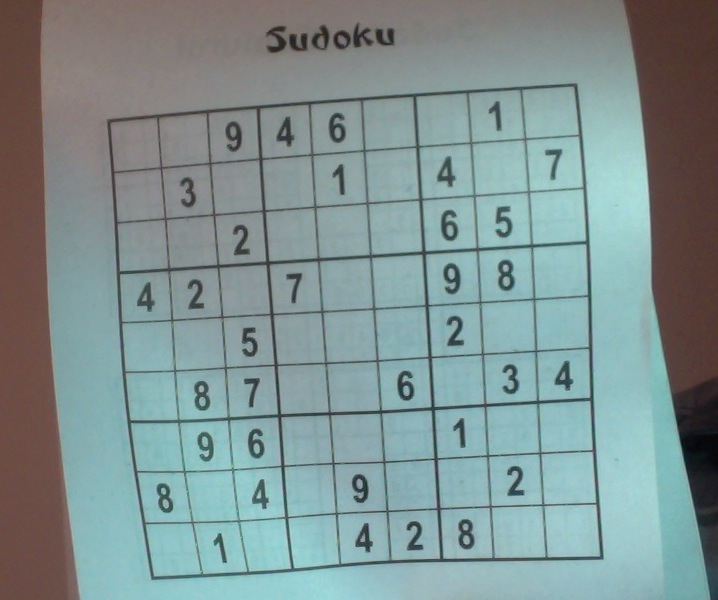
\includegraphics[width=.5\textwidth]{Abbildungen/Input}
    \end{center}
    \caption{Das verwendete Testbild}
    \label{fig:Input}
\end{figure}

\section{Methodik}
Zum Lösen dieser Aufgabe wird die Programmiersprache \emph{Python 2.7} verwendet.
Für diese steht in Form der Open-Source Library \emph{OpenCV} eine leistungsstarke Bibliothek zur Bildverarbeitung zur Verfügung.
OpenCV selbst ist in C++ geschrieben, bietet jedoch entsprechende Python-Bindings an.

Für die Erkennung der Ziffern wird die von Google entwickelte \emph{Tesseract}-Library verwendet. Auch für diese existieren Python-Bindings in Form von \emph{python-tesseract}.

Als Eingangsbild wird das Bild aus Abbildung~\ref{fig:Input} verwendet. Dieses wurde mit der Webcam eines MacBook Pro aufgenommen.

\subsection{Bild-Vorverarbeitung}
Das Bild wird zunächst in Graufstufen umgesetzt, da Farben vernachlässigt werden können.

Anschließend wird das Bild mit einem adaptiven Threshold binärisiert. Ein einfacher Threshold eignet sich nicht, da die Licht- und Kontrastverhältnissen unbekannt sind.

Um das Rauschen zu entfernen, wird das Bild mit einem 3x3 Medianfilter gefiltert.

\begin{figure}[h!]
    \subfigure{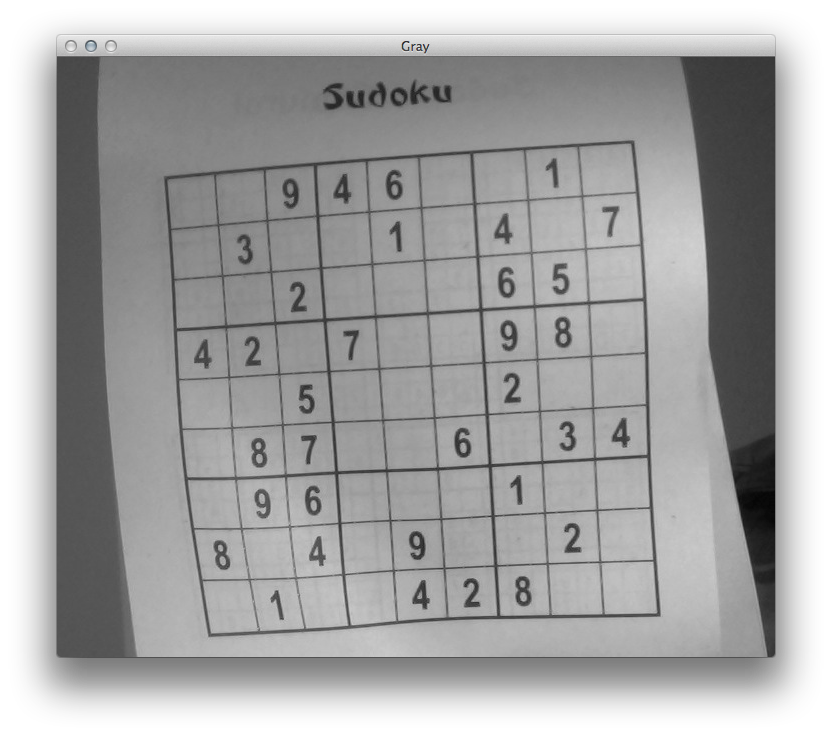
\includegraphics[width=0.49\textwidth]{Abbildungen/gray}}
    \subfigure{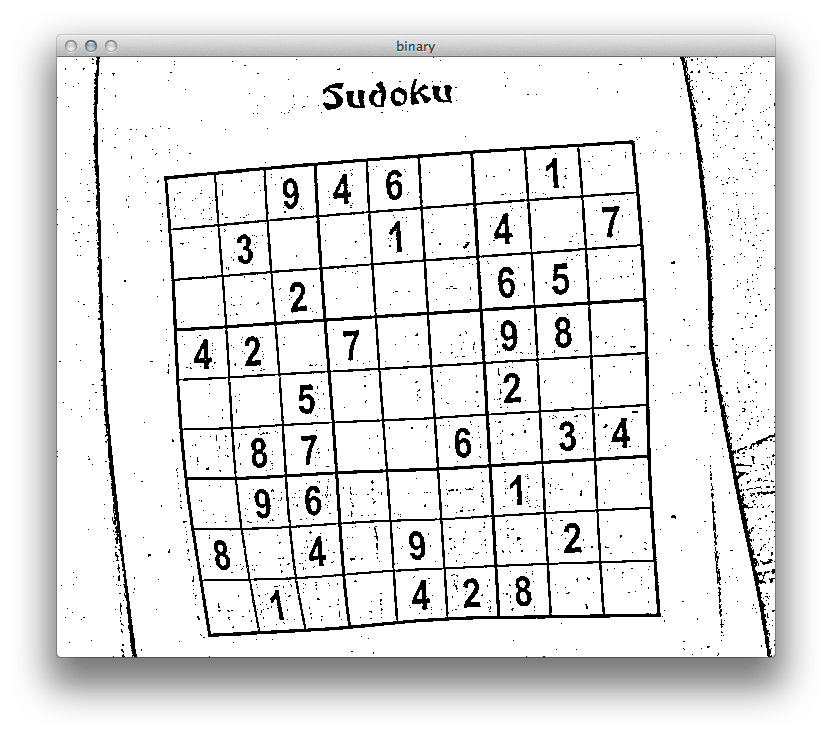
\includegraphics[width=0.49\textwidth]{Abbildungen/binary}}
    \hfill
    \caption{Verlängerte und binärisierte Kanten}
\end{figure}

\begin{figure}[h!]
    \begin{center}
        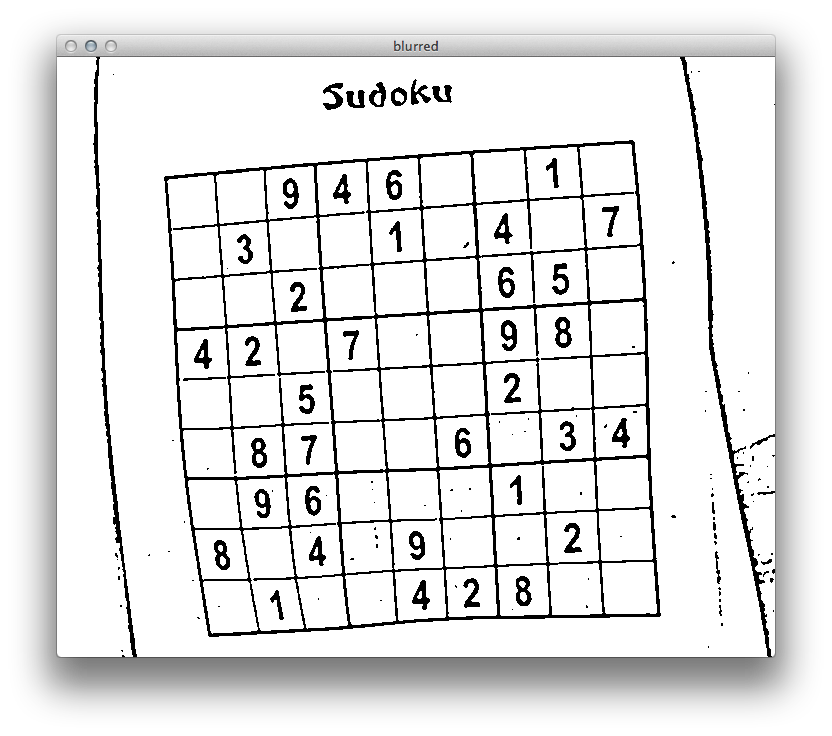
\includegraphics[width=.5\textwidth]{Abbildungen/median}
    \end{center}
\end{figure}


\subsection{Sudoku lokalisieren}
Um die Position des Sudokus zu bestimmen werden zunächst alle Konturen im Bild ermittelt. Dazu muss das binärisierte Bild invertiert werden, da der Algorithmus weiße Pixel als Objektpixel erwartet.
Alle Konturen werden über folgende Kriterien gefiltert:

\begin{enumerate}
    \item Das umschließende Rechteck muss annähernd quadratisch sein. Dazu werden die Seitenverhältnisse überprüft.
    \item Um kleine Konturen auszuschließen, wird eine Mindestfläche vorgegeben.
    \item Hinzu kommt ein Mindestwert für das Verhältnis der Konturfläche zur Fläche des umschließenden Rechtecks, um beispielsweise ``L''-förmige Konturen auszuschließen.
\end{enumerate}

Von allen Konturen, die diese Bedingungen erfüllen, wird diejenige mit der größten Konturfläche ausgewählt.


\subsection{Sudoku isolieren und transformieren}
Das umschließende Rechteck der Kontur stellt nur in Spezialfällen die tatsächliche Kontur des Sudokus dar.
Um die Eckpunkte des Sudokus im Bild zu ermitteln, wird daher die gefundene Kontur mit einem Linienzug approximiert.
Über Parameter der Funktion lässt sich der maximal gültige Fehler der Approximation einstellen.
So kann erreicht werden, dass die Approximation aus genau vier Punkten besteht, die dann die Eckpunkte darstellen.

Der zulässige Fehler ist abhängig vom Umfang der Kontur.
Er muss so eingestellt werden, dass leichte Verformungen noch zulässig sind, die Ecken aber zuverlässig erkannt werden.

Wenn die Kontur mit vier Punkten approximiert werden konnte, wird zur Separation eine Maske erstellt.
Dazu wird auf einen schwarzen Hintergrund die Kontur des Sudokus gezeichnet und weiß gefüllt.
Dieses Bild wird invertiert und mit dem bereits binärisierten Bild verodert.
Das Resultat ist das isolierte Sudoku auf weißem Hintergrund.
Dies war notwendig, da auf schwarzem Hintergrund die äußerste Feldbegrenzung verschwindet.

\begin{figure}[h!]
    \begin{center}
        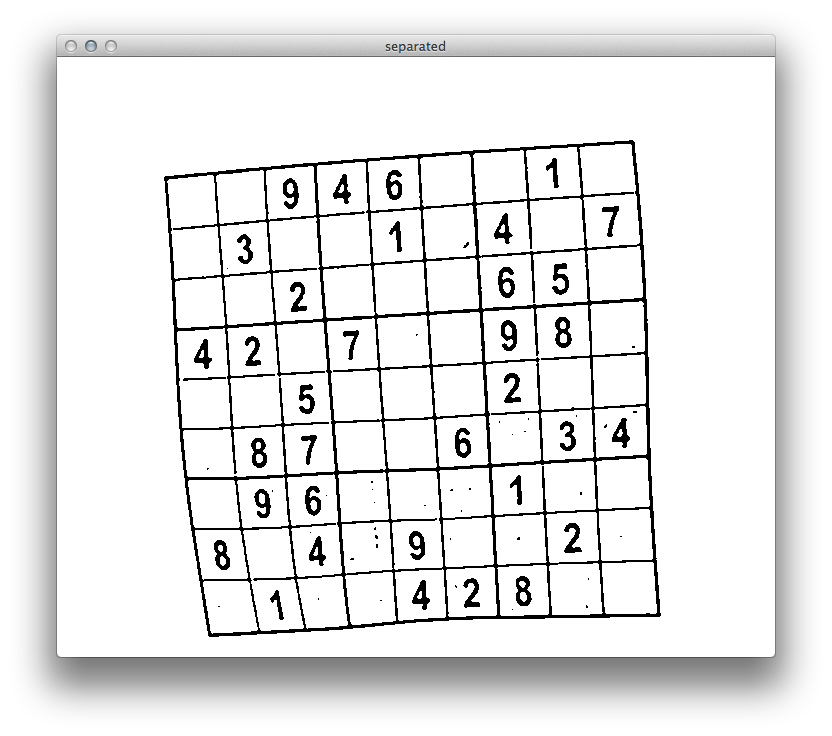
\includegraphics[width=.5\textwidth]{Abbildungen/separated}
    \end{center}
\end{figure}

Das isolierte Sudoku wird anhand der approximierten Eckpunkte perspektivisch zu einem Quadrat der Größe 450x450px transformiert.
Je nach Biegung des Papiers sind im Quadrat und an den Außenrändern noch perspektivische Verzerrungen vorhanden. Um zu verhindern, dass diese verzerrten Randbereiche abgeschnitten werden, wird ein zusätzlicher Abstand von 50px hinzugefügt.

Zuerst werden die Eckpunkte des Zielquadrats festgelegt und den approximierten Eckpunkten zugewiesen. Daraus ergibt sich die Transformationsmatrix, die anschließend auf das isolierte Sudoku angewendet wird.

\begin{figure}[h!]
    \begin{center}
        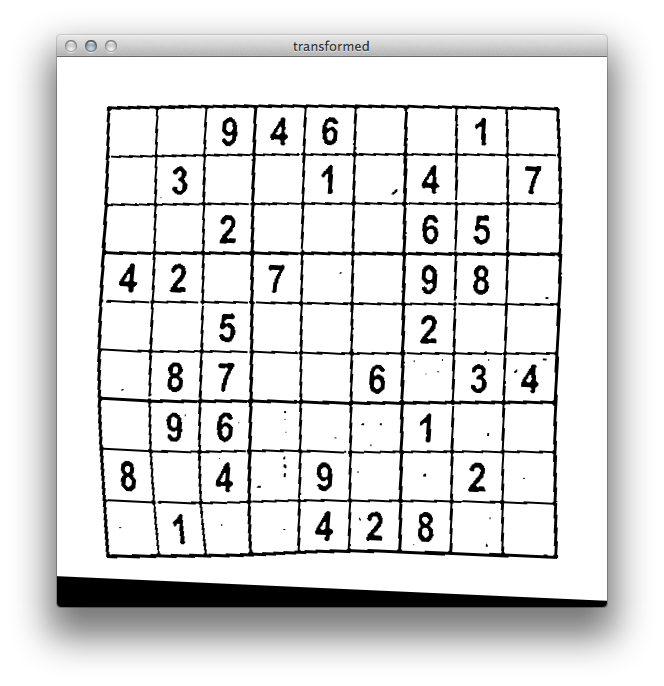
\includegraphics[width=.5\textwidth]{Abbildungen/transformed}
    \end{center}
\end{figure}


\subsection{Gitteranalyse}
Da die Positionen der Ziffern aufgrund der Wölbung des Papiers nicht fix angenommen werden können, müssen zunächst die Eckpunkte der Einzelzellen gefunden werden.
Dazu werden die Kreuzungspunkte der Gitterlinien bestimmt.

\subsubsection{Linienerkennung}
Zur Erkennung der Kanten wird der Sobel-Operator in X- und Y-Richtung eingesetzt.

\begin{figure}[h!]
    \subfigure{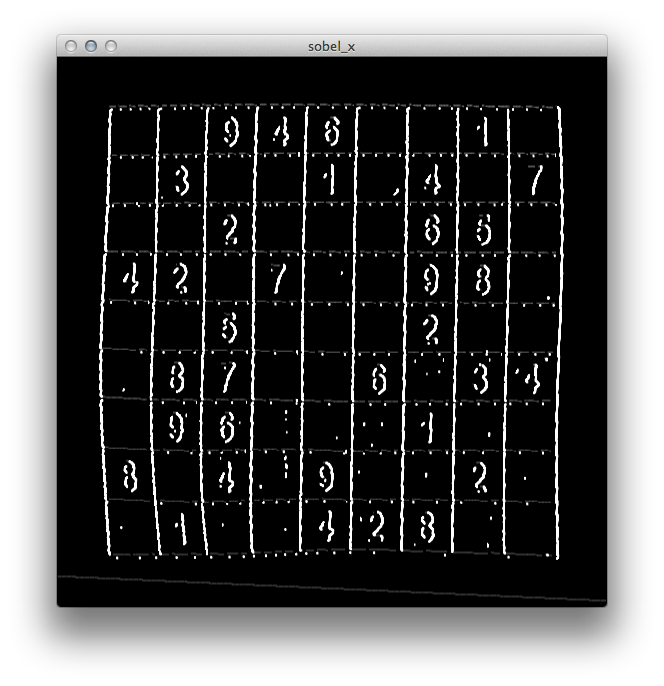
\includegraphics[width=0.49\textwidth]{Abbildungen/sobel_x}}
    \subfigure{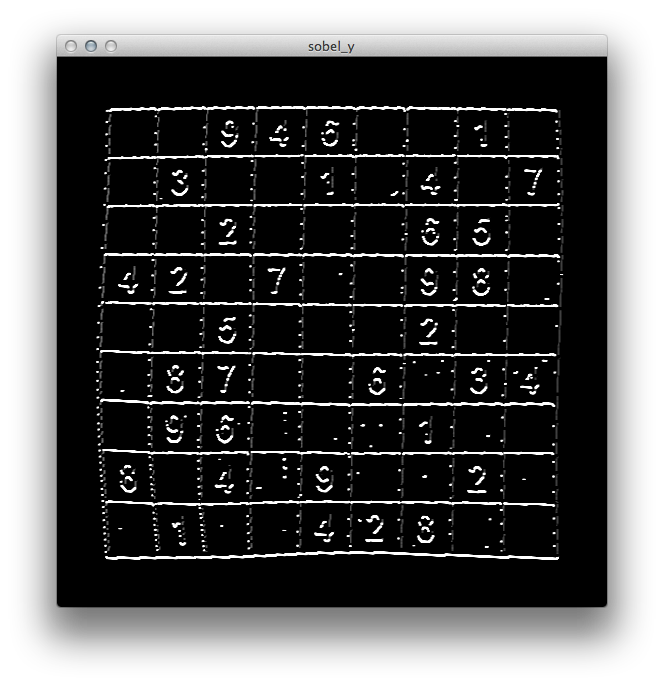
\includegraphics[width=0.49\textwidth]{Abbildungen/sobel_y}}\hfill
    \caption{Erkannte Kanten nach der Sobel-Operation}
\end{figure}

Der Sobel-Operator generiert an den Kreuzungspunkten Fehlstellen, daher sind die Gitterlinien nicht durchgängig und müssen geschlossen werden.
Sie werden durch einen Closing-Operator geschlossen.
Dazu wird das Bild mit dem gleichen Element dilatiert und anschließend erodiert.

Der Sobel-Operator erzeugt Grauwerte im Bild, die durch eine erneute Binärisierung wieder verworfen werden.

\begin{figure}[h!]
    \subfigure{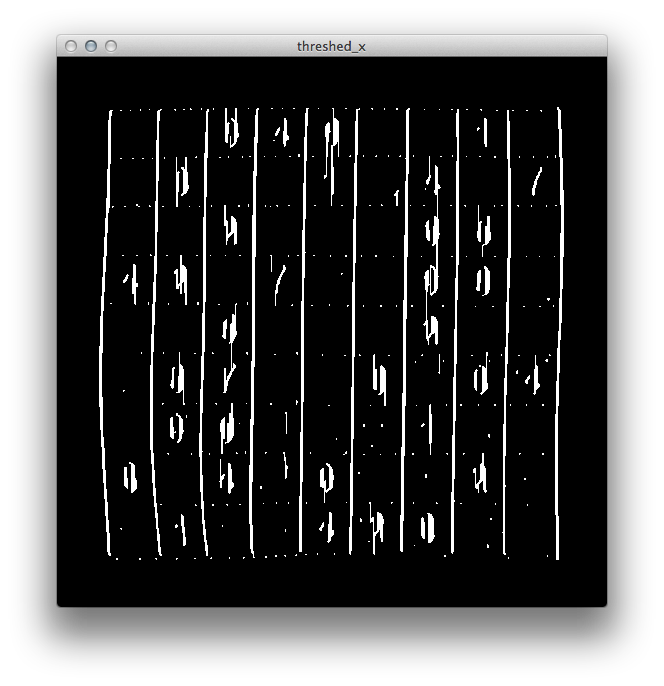
\includegraphics[width=0.49\textwidth]{Abbildungen/threshed_x}}
    \subfigure{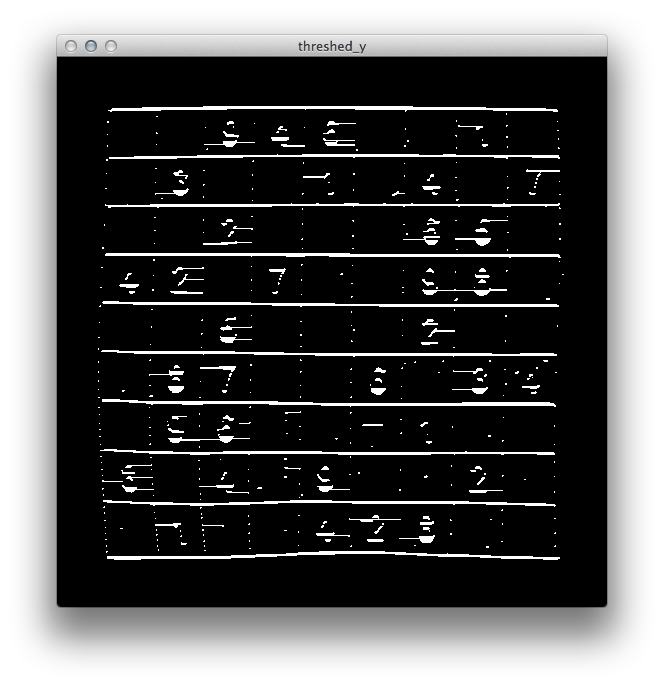
\includegraphics[width=0.49\textwidth]{Abbildungen/threshed_y}}\hfill
    \caption{Verlängerte und binärisierte Kanten}
\end{figure}

Aus diesem Bild werden die zehn größten Konturen ermittelt und isoliert, indem die Konturen der Linien auf ein leeres Bild gezeichnet werden.

\begin{figure}[h!]
    \subfigure[vertikal]{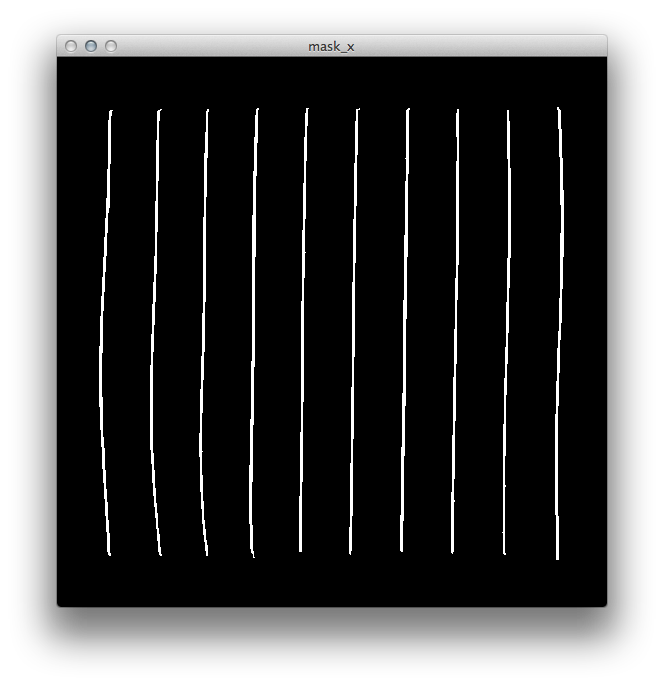
\includegraphics[width=0.49\textwidth]{Abbildungen/mask_x}}
    \subfigure[horizontal]{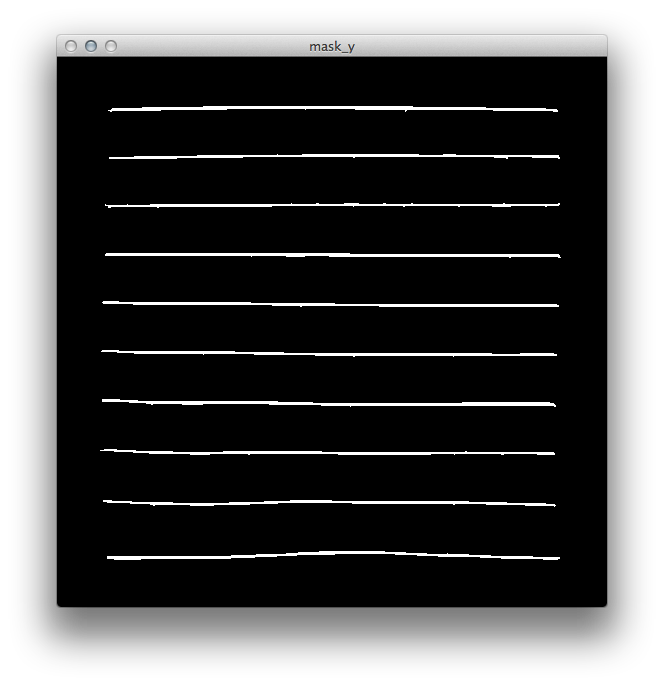
\includegraphics[width=0.49\textwidth]{Abbildungen/mask_y}}\hfill
    \caption{Die vereinzelten Linien}
\end{figure}

Die Linien werden verlängert, damit sichergestellt ist, dass auch an den Randpunkten Überschneidungen entstehen.
Durch Verodern erhält man das vollständige Sudoku-Gitter, durch Verunden nur die Kreuzungspunkte.

\begin{figure}[h!]
    \subfigure[Kreuzungspunkte (nach Verundung)]{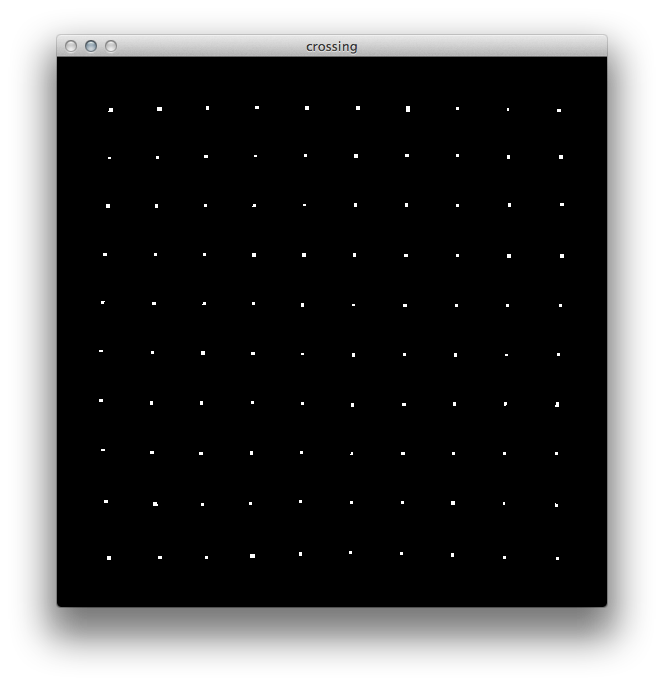
\includegraphics[width=0.49\textwidth]{Abbildungen/crossing}}
    \subfigure[Gitter (nach Veroderung)]{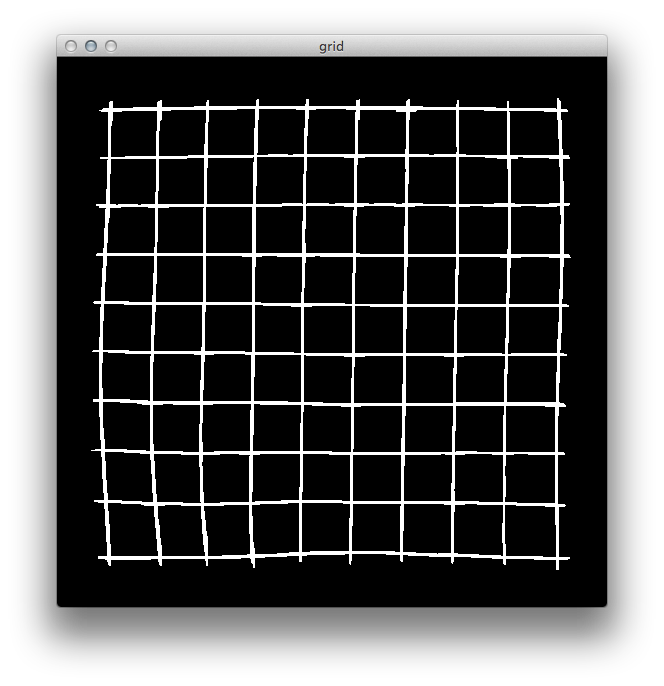
\includegraphics[width=0.49\textwidth]{Abbildungen/grid}}\hfill
    \caption{Erkannte Kreuzungspunkte und Gesamtgitter}
\end{figure}


\subsubsection{Reihenfolge der Kreuzungspunkte}
Wendet man auf das Bild der Kreuzungspunkte eine Konturerkennung an, liegen die erkannten Konturen nicht in einer definierten Reihenfolge vor und müssen daher sortiert werden.

Als Koordinaten der Kreuzungspunkte werden die Mittelpunkte der umschließenden Rechtecke verwendet.
Die Konturpunkte liegen in Form einer eindimensionalen Liste vor. Um diese nach ihrer Position im Bild zu sortieren, müssen die Koordinaten zunächst nach ihrer Y-Position sortiert werden.
Anschließend werden die Koordinaten zu Gruppen zusammengefasst.
Die Gruppengröße entspricht dabei der Anzahl der Koordinaten auf einer Kante des Quadrats, also der Wurzel aus der Anzahl der verfügbaren Punkte.

Innerhalb der Gruppen werden die Koordinaten nun nach ihrer X-Position sortiert und die Gruppen anschließend wieder aufgelöst.

Die Funktionen hierfür kommen aus der Python-Library \emph{numpy}, welche speziell für Matrixoperationen konzipiert wurde.

\begin{figure}[h!]
    \subfigure[unsortiert]{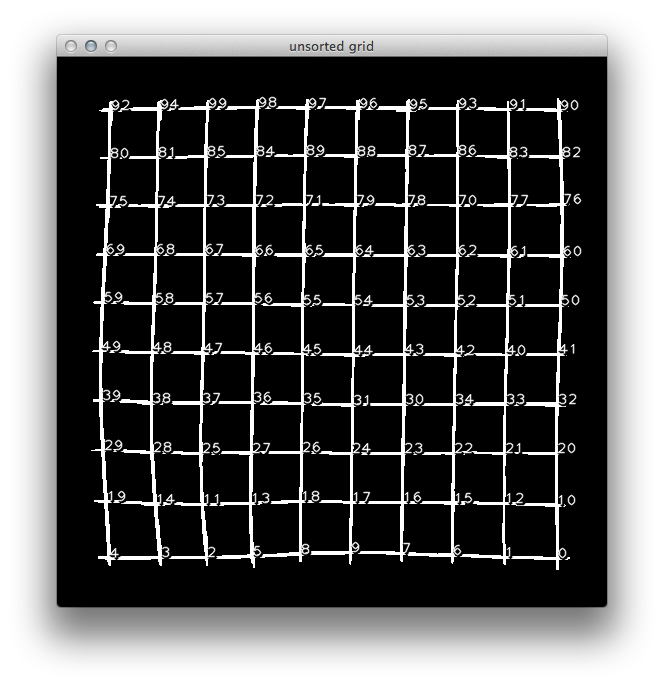
\includegraphics[width=0.49\textwidth]{Abbildungen/unsorted_grid}}
    \subfigure[sortiert]{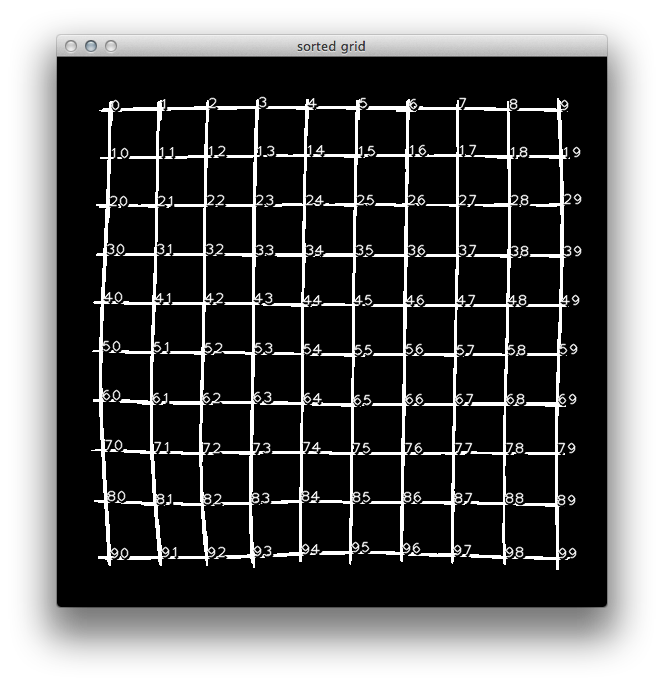
\includegraphics[width=0.49\textwidth]{Abbildungen/sorted_grid}}\hfill
    \caption{Reihen der Kreuzungspunktkoordinaten}
\end{figure}


\subsection{Ziffererkennung}
Für die Ziffererkennung werden zunächst Einzelbilder der Zellen benötigt.

Die Kreuzungspunkte liegen in diesem Schritt bereits sortiert vor.
Als Referenzkoordinate für jede Zelle wird jeweils der obere linke Eckpunkt betrachtet. Alle Eckpunkte auf dem rechten Rand werden ausgelassen.
Ist der obere, linke Eckpunkt einer Zelle gegeben, liegt der rechte obere Eckpunkt eine Position, der untere linke Zehn und der untere rechte Elf Positionen weiter in der Liste der Kreuzungspunkte.

Sobald die Eckpunkte einer Zelle bekannt sind, werden diese perspektivisch zu einem Quadrat transformiert, wobei die fehlerbehafteten Randbereiche abgeschnitten werden.

\begin{figure}[h!]
    \begin{center}
        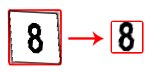
\includegraphics[]{Abbildungen/Ziffer}
    \end{center}
\end{figure}

Die so isolierten Ziffern werden der OCR-Library Tesseract übergeben.
Diese wurde so initialisiert, dass sie ein einzelnes Zeichen erwartet. Außerdem wurde die Liste der zulässigen Buchstaben so modifiziert, dass nur Ziffern von 0-9 erkannt werden können.
Die Library liefert einen String mit dem Ergebnis der Konvertierung zurück.

Um die Fehlerrate zu minimieren, wird das Ergebnis anschließend auf Sinnhaftigkeit überprüft.
Dazu wird zunächst versucht, das Ergebnis in einen Integer zwischen 0 und 9 zu konvertieren.

Schlägt dies fehl, kann es sich um eine Leerzelle handeln.
Wird dennoch eine Kontur mit einer gewissen Mindestgröße gefunden, wird davon ausgegangen, dass eine Zahl vorhanden war, aber nicht richtig erkannt wurde.
In diesem Fall wird der Vorgang abgebrochen und auf den nächsten Frame gewartet.

Die erkannten Ziffern werden anschließend in das Ausgangsbild hineingeschrieben.

\begin{figure}[h!]
    \begin{center}
        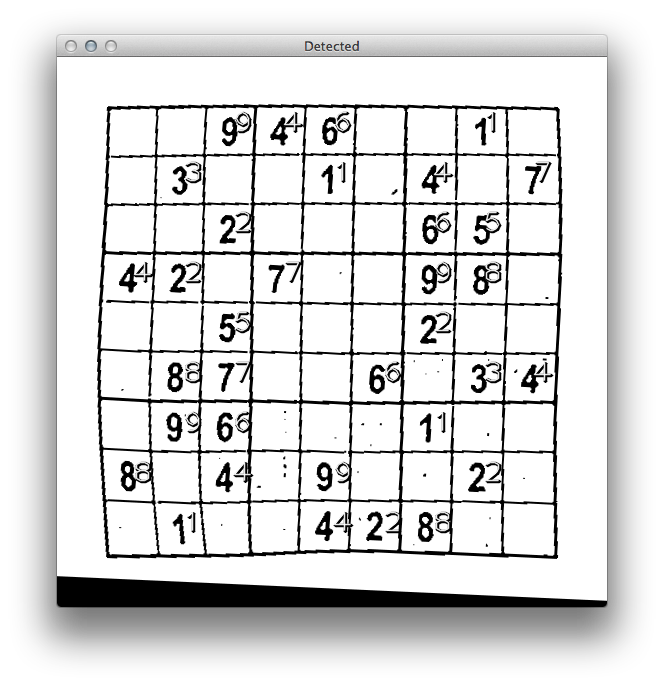
\includegraphics[width=.5\textwidth]{Abbildungen/detected}
    \end{center}
\end{figure}



\subsection{Lösung des Sudokus}
